\documentclass[11pt, a4paper]{article}
\usepackage{polski}
\usepackage[UTF8]{inputenc}
\usepackage{amsmath}
\usepackage{longtable}
\usepackage[pdftex]{graphicx}
\usepackage{wrapfig}

\usepackage[bookmarksnumbered,colorlinks,plainpages,backref]{hyperref} %wersja CD
\hypersetup{
 citecolor=[rgb]{0, 0.6, 0},
 linkcolor=[rgb]{0.8,0,0},
 urlcolor=blue}


\author{K.~Narożnik}
\title{Krótko o FC Barcelonie}
\date{08.12.2014}
\linespread{1.4}

\linespread{1.2}
\begin{document}
\maketitle

\newpage
\tableofcontents
\newpage

\section{Ogólnie o Barcelonie}
\label{sec:Ogolnie}

Futbol Club Barcelona (w języku katalońskim), w skrócie Barca – kataloński wielosekcyjny klub sportowy, istniejący od chwili założenia drużyny piłkarskiej. Założony w X przez grupę Szwajcarów, Anglików i Hiszpanów, z czasem stał się katalońską instytucją o dużym znaczeniu społecznym. Jedna z wielu teorii mówi, że barwy klubowe Barcelona zaczerpnęła od szwajcarskiego klubu FC Basel.

Drużyna piłkarska należy do najbardziej utytułowanych zespołów świata w tej dyscyplinie – ma na koncie dwadzieścia dwa mistrzostwa Hiszpanii, dwadzieścia sześć Pucharów Króla Hiszpanii, dziesięć Superpucharów Hiszpanii, cztery Puchary Europy, cztery Puchary Zdobywców Pucharów, cztery Superpuchary Europy, dwa razy Klubowe Mistrzostwo Świata/Puchar Interkontynentalny i wiele innych trofeów.

Klub ma 162 979 socios – członków klubu – i miliony culés na całym świecie, z których część zrzeszona jest w penyach, czyli oficjalnych fanklubach, których jest 1054. Posiada również rozbudowaną infrastrukturę – stadiony Camp Nou, Mini Estadi, miasteczko sportowe Ciutat Esportiva Joan Gamper, szkółkę La Masía i halę Palau Blaugrana, w której rozgrywają swoje mecze zawodnicy innych sekcji.

Poza sekcją piłkarską do FC Barcelona należą jeszcze: Regal FC Barcelona, FC Barcelona-Intersport, FC Barcelona Sorli Discau i FC Barcelona Senseit). Klub posiada także rezerwową i młodzieżową drużynę piłki nożnej (FC Barcelona B), a także liczne sekcje amatorskie.

Drużyna z Camp Nou na arenie międzynarodowej startuje nieprzerwanie od 50 lat, czyli od początku powstania europejskich pucharów. Jest jednym z trzech klubów, które od założenia Primera División, czyli od 1929 roku, nieprzerwanie grają w najwyższej klasie rozgrywkowej Hiszpanii.
\section{Matma w Barcelonie}
\label{sec:Matma}
Cóż, Barca ma też stały wzór na liczbę punktów pod koniec sezonu. Jest on taki:
$$\frac{liczba~symulek~Neymara}{bramki~CR7} * {ugryzienia~Suareza}$$
Można też policzyć to inaczej, bo układem równań z innymi zmiennymi, gdzie y to miejsce pod koniec sezonu :
\begin{equation}
	y = \left\{	
	\begin{array}{ll}
	odbiory~Busquetsa & \textrm{jeżeli $odbiory > 0 \land CR7 <0$} \\
	sprinty~Pique & \textrm{jeżeli $sprinty > 0 $} \\
	1 & \textrm{gdy Messi strzeli więcj niż 40 goli}
		
	\end{array} \right.
	\label{eq:nr1}
\end{equation}
\section{Piłkarze Barcelony}
\label{sec:Pilkarze}
\begin{longtable}{|l|r|r|r|}
\caption{Piłkarze Barcelony}\\\hline
\multicolumn{4}{|c|}{Wybrani piłkarze sezonu 2014/15}\\\hline
imie & nazwisko & mecze & gole \\ \hline
\endfirsthead
\hline
\multicolumn{4}{|c|}{Wybrani piłkarze sezonu 2014/15}\\
imie & nazwisko & mecze & gole \\ \hline
\endhead
\hline \multicolumn{4}{|c|}{Wybrani piłkarze sezonu 2014/15}\\ \hline
\endfoot
\hline \multicolumn{4}{|c|}{Wybrani piłkarze sezonu 2014/15}\\
\hline
\endlastfoot
Martin & Montoya & 1 & 0 \\
Gererd  & Pique & 12 & 1 \\
Marc & Bartra & 5 & 0 \\
Lionel & Messi & 13 & 20 \\
Luis  & Suarez & 6 & 0 \\
Claudio & Bravo & 13 & 0 \\
Jordi & Alba & 13 & 1 \\
Munir  & El Haadi & 4 & 1 \\
Sandro & Ramires & 2 & 2 \\
Jordi & Masip & 0 & 0 \\
Marc-Andre  & Ter Stegen & 6 & 1 \\
Andres & Iniesta & 9 & 2 \\
\end{longtable}
\section{Najnowsze informacje o Barcelonie}
\begin{wrapfigure}{r}{0.5\textwidth}
\begin{center}
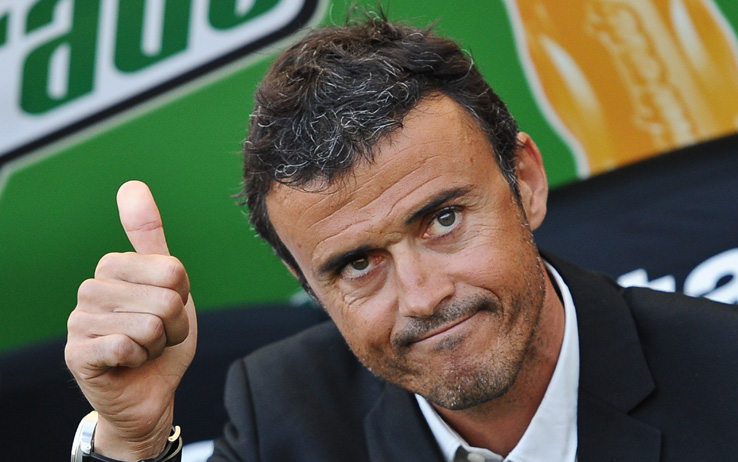
\includegraphics[width=0.48\textwidth]{luzienrique.jpg}
\end{center}
\caption{Luiz Enrique\cite{99}}
\label{img:Luiz}
\end{wrapfigure}
Najnowsza historia Barcy optymistyczna nie jest. Trenerem od nowego sezonu został Luiz Enrique.
16 maja 2014 roku Enrique ogłosił, że opuszcza Celtę Vigo. Dwa dni później podpisał dwuletni kontrakt z Barceloną. Jednak drużyna nie gra, tak, jakby oczekiwali kibice i coraz więcej jest głosów ay podziękowac za współpracę wychowankowi Barcelony.

\section{Inne, nie wiem gdzie indziej wstawić}
\begin{figure}[!ht]
\centering
\setlength{\unitlength}{0.75mm}
\begin{picture}(60,40)
\put(20,20){\vector(2,0){30}}
\put(10,20){\vector(2,1){25}}
\put(30,20){\vector(3,1){10}}
\put(40,20){\vector(3,1){10}}
\put(25,20){\vector(1,2){15}}
\thicklines
\put(15,20){\vector(-4,1){16}}
\put(19,20){\vector(-1,4){5}}
\thinlines
\put(30,20){\vector(-1,-4){5}}
\end{picture}
\caption{Coścoś}
\label{fig:strzaleczki}
\end{figure}

\newpage
\bibliographystyle{plain}
\begin{thebibliography}{9}
\bibitem{99}  ASD : \emph{http://pl.wikipedia.org/wiki/Luis\_Enrique}

\end{thebibliography}
\end{document} 